\section{Generic two-wind bow shock model}
\label{sec:generic-model}

\begin{figure}
% 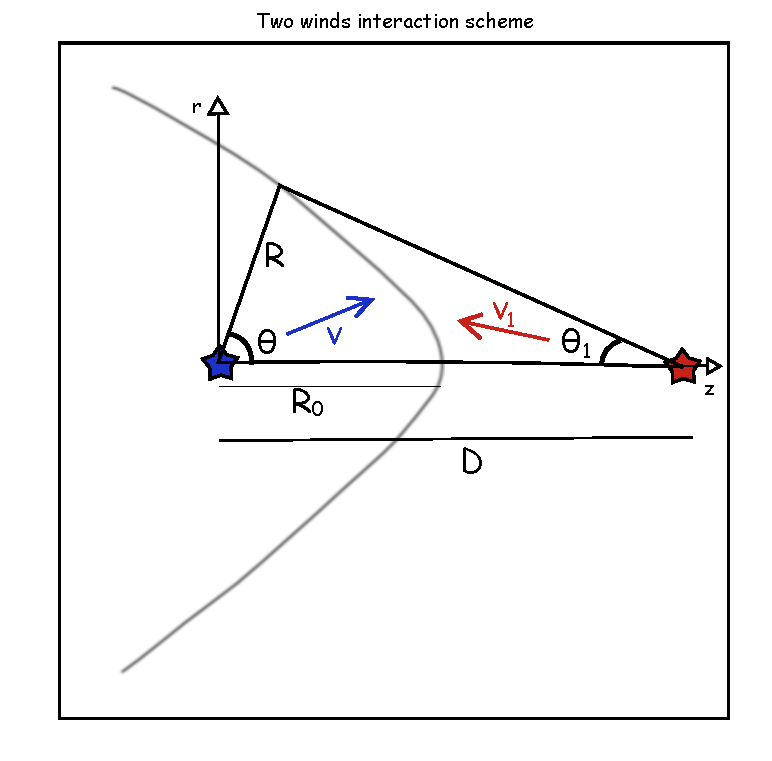
\includegraphics[width=\linewidth]{2winds-scheme}
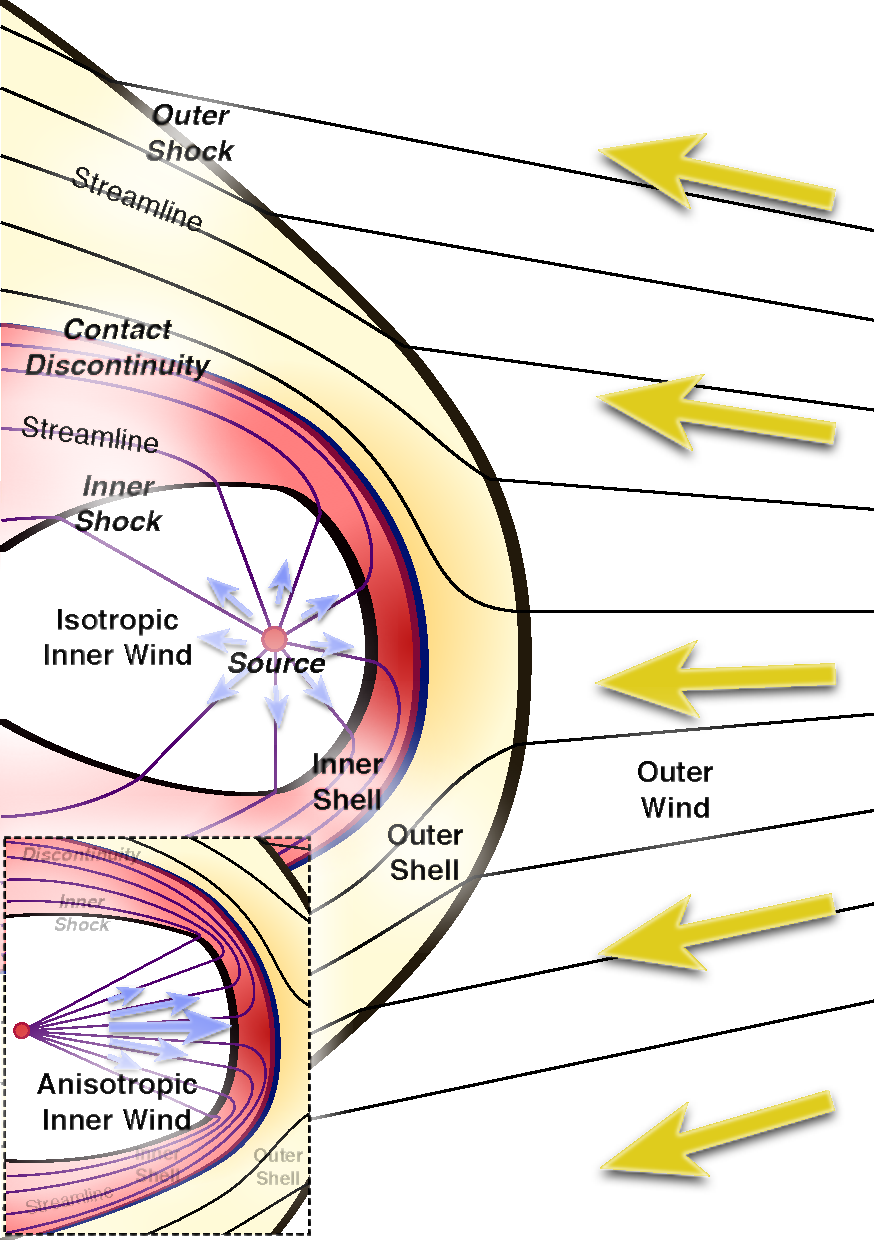
\includegraphics[width=\linewidth]{figs/generic-bowshock}
\caption{Quasi-stationary bow shock structure formed by the
  interaction of two supersonic winds.  Lower-left inset box shows the
  case where the inner wind is anisotropic.   
  % the two winds problem. Any point in the shell is located with the
  % coordinates $(R,\theta)$, and $\theta_1$ is measured from the
  % external wind position
}
\label{fig:2-winds}
\end{figure}

The general case of a two-wind interaction bow shock is illustrated in
Figure~\ref{fig:2-winds}.  If the winds are isotropic, then the bow
shock pattern wraps around the weaker of the two sources, in 

The bow shocks we consider are originated by a source located at the origin, emitting a wind with a mass loss rate of $\dot{M}_w$ and a terminal
(supersonic) velocity $v_w$. This wind interacts with another wind originated by another source located at a distance $D$ from the first one. 
The mass loss rate of the second source is $\dot{M}_{w1}$ and the terminal velocity is $v_{w1}$. The momentum of the wind of the second source is
higher than the momentum of the first one, and the resultant bow shock is stationary due to pressure balance. 

\subsection{Characteristic Radii}

In order to contrast different bow shock models, we  derive a set of measurable radii. Each model used should predict them and these predictions can be
compared with observations.

\begin{itemize}
\item Radius at axis of symmetry. Denoted as $R_0$. 
\item Radius of Curvature at the axis of symmetry. Denoted as $R_c$
\item Radius at the  perpendicular direction to the symmetry axis. Denoted as $R_{90}$
\item For open bow shocks, the asymptotic angle. Denoted as $\theta_\infty$
\end{itemize} 

\begin{figure}
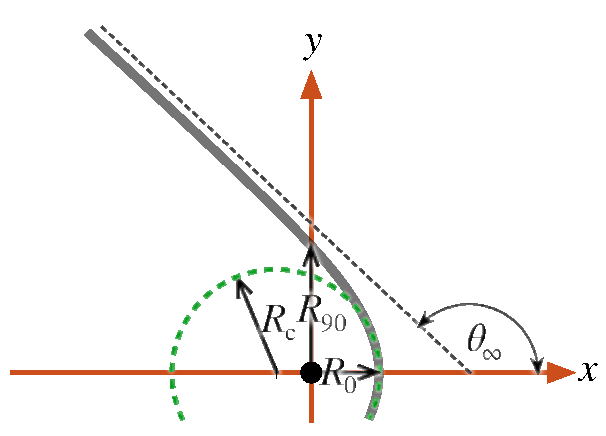
\includegraphics[width=\linewidth]{figs/characteristic-radii}
\caption{Schematic representation of the characteristic radii $R_0$, $R_{90}$ and the radius of curvature at the symmetry axis $R_c$}
\end{figure}



%%% Local Variables:
%%% mode: latex
%%% TeX-master: "quadrics-bowshock"
%%% End:
